\chapter{Transformers e Vision Transformers}
\label{appendice_transformers}
Questa appendice è dedicata a dettagliare maggiormente temi riguardanti transformers e vision transformers (ViT). In particolare, il ViT è la rete che ricopre il ruolo di encoder nell'architettura di DINOv2 (Figura \ref{fig:arch_dinov2}) e i quali outputs utilizziamo in fase di sperimentazione. Si andranno ad esporre gli aspetti concettuali e l'intuizione dietro il funzionamento dei due, senza scendere nel dettaglio algebrico.

L'introduzione dei transformers nel 2017 ha cambiato il panorama della ricerca in ambito di \textit{natural language processing}, e non solo. Questo nuovo approccio all'intelligenza artificiale, in combinazione con altri fattori come l'aumento della disponibilità e potenza di calcolo delle GPU, ha portato negli ultimi anni ad una rivoluzione che ci ha condotti fino a modelli moderni come GPT, superando le performance di tradizionali approcci di deep learning.

\section{Transformers}
I transformers vengono introdotti per la prima volta nel 2017 dal paper "\textit{\citefield{transformer}{title}}" \cite{transformer}. Questa nuova rete si basa interamente sul concetto di \textit{attention}, applicato al task di traduzione dall'inglese al tedesco.

\begin{figure}[ht]
    \centering
    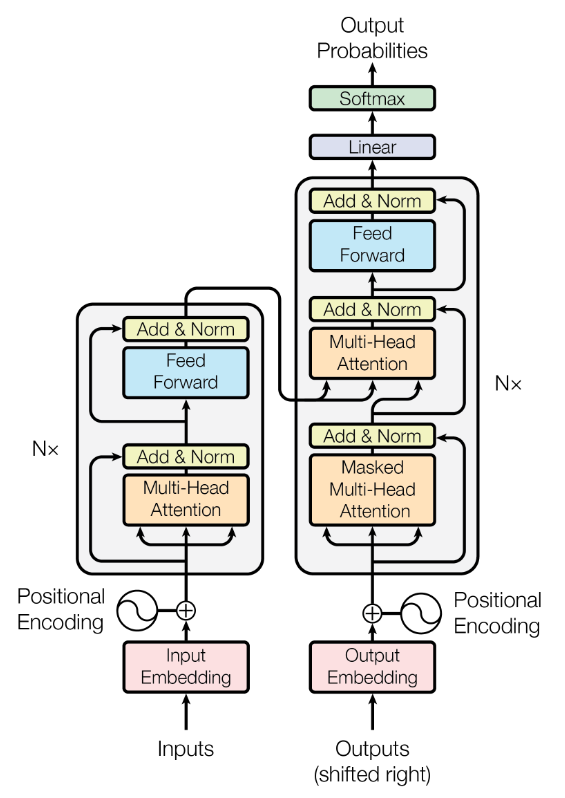
\includegraphics[height=12cm]{Immagini/transformers/arch_transformer.png}
    \caption{Architettura di un transformer.}
    \label{fig:arch_transformer}
\end{figure}

La struttura di un transformer è illustrata in Figura \ref{fig:arch_transformer}. Si compone di un insieme di \textit{encoders}, seguiti da un insieme \textit{decoders}. Generalmente, il numero di encoders e decoders scelto è di 6 ciascuno, ma c'è spazio per la sperimentazione. Il blocco di encoders ha il compito di trasformare una sequenza di embeddings \((x_1, \dots, x_n)\), che identificano la sequenza di tokens della frase, in una sequenza di rappresentazioni \(z = (z_1, \dots, z_n)\). Il blocco di decoding, invece, a partire da \(z\) genera in output una sequenza di simboli \((y_1, \dots, y_m)\). Questo viene fatto mappando il vettore di features prodotto dal decoder in un nuovo vettore, lungo quanto il numero di parole nel dizionario di vocaboli che la rete è in grado di predirre, tramite un layer lineare, e utilizzando un softmax per scegliere quale sia la parola più probabile a seguire quella correntemente analizzata. Ad ogni step successivo, il modello consuma i simboli precedentemente generati come input aggiuntivo nel generare altro testo. La loss utilizzata è una cross-entropy.

\subsection{Preparare l'input}
Data una frase da tradurre, questa viene suddivisa in \textit{tokens}, che possono essere una singola parola, parti di frasi, punteggiatura. Ciascuno di essi viene trasformato in un vettore numerico univoco per poter essere passato alla rete. Questa traduzione può essere fatta tramite approcci come \textit{word2vec} (\cite{word2vec}), che consiste in una rete neurale poco profonda allenata a mappare parole in uno spazio continuo in cui parole simili sono vicine fra loro.
Al vettore risultante viene poi aggiunto un ulteriore vettore, detto \textit{positional encoding}, che codifica la posizione del token nella frase. Questo è importante, in quanto i transformers processano tutti i tokens parallelamente, che è una delle forze di questa architettura, ma questo cancella la nozione naturale di ordine delle parole nella frase.

\subsection{Encoder}
Ogni encoder si compone di 2 sublayers. Il primo è un blocco di \textit{self-attention}, mentre il secondo è una semplice rete fully-connected. Viene utilizzata anche una connessione residuale attorno a ciascuno dei due sublayers, seguita da una layer normalization, la quale ha lo scopo di migliorare velocità e stabilità del training, normalizzando le attivazioni ricevute lungo la dimensione delle features. L'output di ogni sotto-layer è quindi \(\text{LayerNorm}(x + \text{Sublayer}(x))\), dove \(\text{Sublayer}(x)\) è la funzione implementata dal sublayer stesso. Questo facilita e stabilizza l'addestramento, mitigando fenomeni come il \textit{vanishing gradient}, quando il gradiente diventa troppo piccolo per permettere apprendimento significativo. Tutti gli outputs, e anche gli embeddings, sono vettori di dimensione 512. 

\subsection{Decoder}
Il decoder si compone a sua volta degli stessi due sublayers di cui si compone l'encoder, fra i quali se ne inserisce un terzo adibito a ricevere e calcolare la self-attention dell'output dell'encoder. Le connessioni residuali vengono mantenute. 

Se nell'encoder l'input del primo sublayer era la frase da tradurre, tokenizzata e trasformata in embeddings, nel decoder l'input è costituito dalla frase già tradotta, che segue gli stessi passi di trasformazione in vettore continuo prima di entrare nella rete. Per questo motivo, il sublayer che lo riceve deve effettuare un mascheramento della frase, in particolare degli embeddings dei tokens che ancora non sono stati predetti dalla rete (si pongono a \(-\infty\)). Questo evita che la rete possa conoscere quale sia il risultato della predizione del token corrente prima ancora di averla effettuata, assicurando che una predizione in posizione \(i\) dipenda solo dai token di output precedenti a \(i\). È necessario fornire alla rete le traduzioni corrette per i tokens già predetti, in fase di training, per evitare che gli errori di predizione per tokens iniziali nella frase possano propagarsi anche a parole successive, portando a prestazioni pessime.

\subsection{Self-attention}
\label{self-attention}
La \textit{self-attention} è il meccanismo attraverso il quale la rete è in grado di concentrarsi su parti specifiche della frase, assegnando un diverso peso a diversi tokens in base alla loro rilevanza al fine di comprendere il significato del testo. Permette di analizzare le \textbf{dipendenze fra parole} tenendo conto delle \textbf{relazioni semantiche e sintattiche}, indipendentemente dalla loro posizione della sequenza.
Il calcolo è il seguente:
\[\text{Attention}(Q, K, V) = softmax(\frac{Q K^T}{\sqrt{d_k}})V\]
dove \(Q\) (query), \(K\) (key) e \(V\) (value) corrispondono allo stessa matrice di embeddings di input, nel primo sublayer, o all'output ricevuto dagli strati precedenti altrimenti. Sostanzialmente, si fa una somma pesata di \(V\), dove il peso è dato dalla compatibilità fra \(Q\) e \(K\), la compatibilità fra una parola e tutte le altre parole nella frase, quanto strettamente siano in relazione fra loro. Il valore di compatibilità viene scalato da un fattore \(\sqrt{d_k}\), che corrisponde alla radice della dimensione del vettore degli embeddings, che aiuta a stabilizzare il calcolo dei pesi.
A livello matematico, il risultato dell'operazione sarà una matrice la cui \(i\)-esima riga esprime quanto il token \(i\)-esimo sia correlato a ciascuno degli altri tokens nella frase. Valori più alti corrispondono a un rapporto più significativo fra i due tokens. 

\subsection{Multi-head attention}
Si introduce anche un meccanismo di \textit{multi-head attention}. Viene realizzando \textbf{ripetendo parallelamente il calcolo della self-attention} un numero \(h\) di volte e introducendo un layer lineare di proiezione per ciascun \(Q, K, V\), con pesi diversi e appresi in training. Gli output di ciascun blocco self-attention vengono poi concatenati fra loro e il risultato viene moltiplicato per un'altra matrice di pesi aggiornata durante la back-propagation, prima di continuare verso il sublayer di aggiunta dei residui e layer normalization.

Il motivo per cui viene utilizzata questa tecnica è che utilizzando più teste di attention, il modello può considerare diverse rappresentazioni contemporaneamente, ognuna che pone attenzione su diverse parti della sequenza. All'interno di una frase, una testa potrebbe concentrarsi sul rapporto fra soggetto e verbo, mentre un'altra testa potrebbe concentrarsi sul rapporto fra soggetto e aggettivi ad esso correlati, e così via. Permette alla rete di comprendere contesti complessi.

\begin{figure}[t]
    \centering
    \subcaptionbox{}{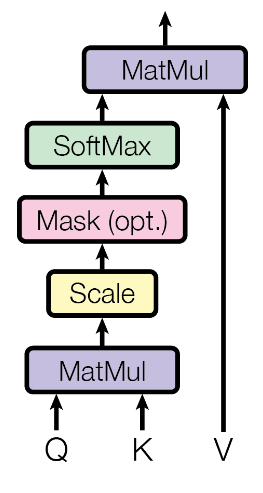
\includegraphics[height = 60mm]{Immagini/transformers/scaled_dot.png}}
    \hspace{5mm}
    \subcaptionbox{}{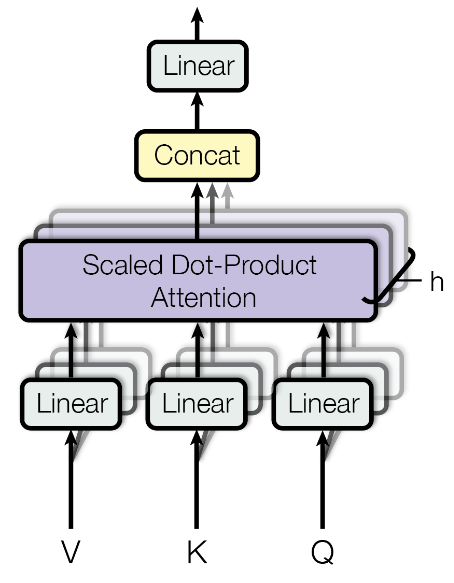
\includegraphics[height= 60mm]{Immagini/transformers/multihead_attention.png}}
    \caption{Workflow per il calcolo della self-attention: (a) scaled dot-product attention, (b) multihead-attention}
    \label{fig:attention}
\end{figure}

\section{Vision Transformers (ViT)}
\label{vit}
I \textit{vision transformers} \cite{vit} nascono nel 2020 dall'osservazione che il concetto di transformer può essere sfruttato anche in ambito di computer vision, su task di image classification, e competere con le prestazioni di modelli tradizionali come le CNN. Si tenta di applicare la stessa struttura del transformer, come descritto da \cite{transformer}, ad un workflow che come input prevede delle immagini, apportando il minor numero di modifiche possibili. Questo viene fatto \textbf{suddividendo} ciascuna \textbf{immagine} in un \textbf{insieme di patches} di dimensione fissa e fornendo in input alla rete una sequenza di embeddings rappresentanti ciascun patch. Queste rappresentazioni saranno trattate allo stesso modo dei tokens utilizzati in NLP e prodotte da un layer lineare.

\begin{figure}[ht]
    \centering
    \subcaptionbox{}{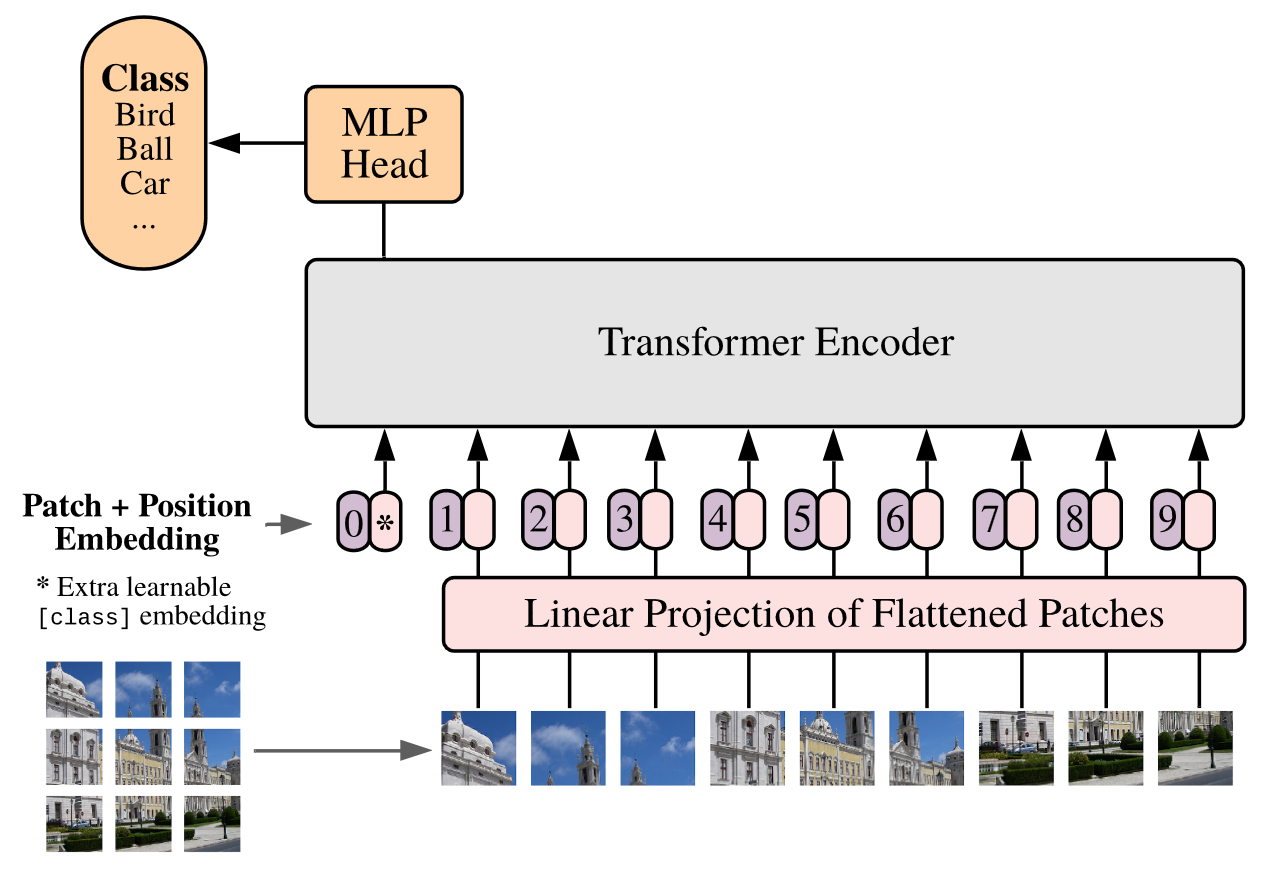
\includegraphics[height=70mm]{Immagini/transformers/arch_vit.png}}
    \subcaptionbox{}{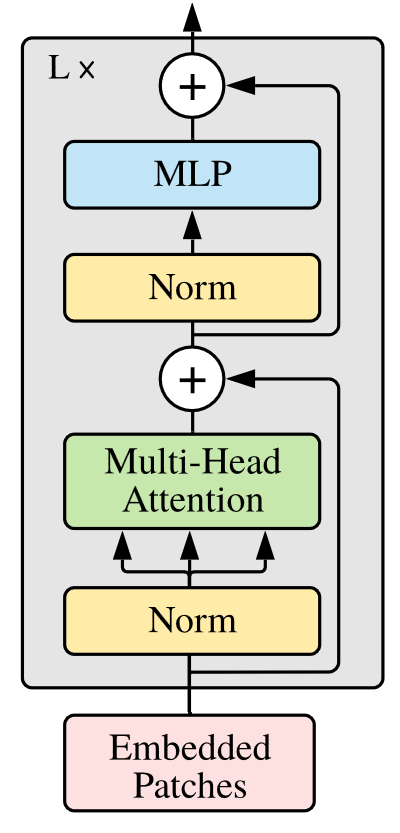
\includegraphics[height=70mm]{Immagini/transformers/encoder_vit.png}}
    \caption{(a) Architettura di un ViT, (b) Encoder}
    \label{fig:arch_vit}
\end{figure}

\subsection{Token [CLS]}
\label{cls}
Una novità introdotta dai ViT rispetto ai transformers è l'aggiunta del \textbf{token [CLS]}, teorizzata prima ancora da BERT \cite{bert}. [CLS] è un token \textbf{completamente appreso} durante l'addestramento della rete, che viene \textbf{aggiunto all'inizio della sequenza di patches di input}. Durante il passaggio attraverso i livelli del transformer, [CLS] interagisce con gli altri tokens tramite il meccanismo di self-attention, e durante questo processo \textbf{accumula informazioni globali riguardo l'intera immagine}. Di fatto, il suo ruolo è quello di aggregare le informazioni racchiuse nella sequenza di patches. Una differenza importante nell'architettura dei ViT rispetto ai transformers è l'assenza di un decoder, essendo l'obiettivo della rete quello della image classification, e non di generare del nuovo contenuto. Per questo, si sceglie di attacare un MLP proprio all'output di [CLS], grazie alla sua caratteristica di sintesi dell'immagine. La testa di proiezione mappa il vettore ricevuto su un nuovo vettore di attivazioni grande quanto il numero di classi da riconoscere, a cui si applica un softmax e la loss scelta.

\subsection{Attention}
Il concetto di attention rimane il nucleo su cui si fonda anche il ViT. Se nel transformer serviva a individuare le relazioni fra tokens all'interno della frase, in questo caso permette di rilevare il rapporto fra patches nell'immagine. Anche in questo caso, per ottenere le mappe di self-attention (Figura \ref{fig:dino_attention}) si deve accedere ad una matrice all'interno della quale la \(i\)-esima riga rappresenta quanto l'\(i\)-esimo patch è correlato a tutti gli altri patch in cui è suddivisa l'immagine. Ad esempio, nella riga 0 troviamo al self-attention riferita al patch [CLS].

\subsection{Tipologie}
\label{tipologie_vit}
Esistono diversi tipi di ViT:
\begin{itemize}
    \item ViT-S (small):
    \begin{itemize}
        \item Numero di \textit{transformer blocks}: 12
        \item Dimensione del vettore di embeddings: 384
        \item Numero di self-attention heads: 6
    \end{itemize}
    \item ViT-B (base):
    \begin{itemize}
        \item Numero di \textit{transformer blocks}: 12
        \item Dimensione del vettore di embeddings: 768
        \item Numero di self-attention heads: 12
    \end{itemize}
    \item ViT-S (large):
    \begin{itemize}
        \item Numero di \textit{transformer blocks}: 24
        \item Dimensione del vettore di embeddings: 1024
        \item Numero di self-attention heads: 16
    \end{itemize}
\end{itemize}
Con il numero di transformer blocks si intende il numero di encoders che formano la rete, come visto in Figura \ref{fig:arch_transformer}. Inoltre, con la notazione ViT/\(N\) si specifica le immagini di input vengono suddivise in patch di dimensione \(N \times N \) pixels.